\documentclass[10pt]{beamer}

\mode<presentation> {

% \usetheme{Berlin}  % Squares
\usetheme{Madrid}  % Circles & dense
% \usetheme{Frankfurt}  % Cirles

\setbeamertemplate{headline}{%
\leavevmode%
  \hbox{%
    \begin{beamercolorbox}[wd=\paperwidth,ht=2.5ex,dp=1.125ex]{palette quaternary}%
    \insertsectionnavigationhorizontal{\paperwidth}{}{\hskip0pt plus1filll}
    \end{beamercolorbox}%
  }
}

\setbeamertemplate{navigation symbols}{}  % To remove the navigation symbols from the bottom of all slides uncomment this line
\setbeamertemplate{items}[circle]

% \useoutertheme{miniframes}
% \useinnertheme{circles}

}

\usepackage{graphicx}
\usepackage{booktabs}
\usepackage{fontspec}
\usepackage{xunicode}
\usepackage{xltxtra}
\usepackage{xecyr}
\usepackage{hyperref}
\usepackage{amsthm}
\usepackage{blindtext}
\usepackage{color}
\usepackage[normalem]{ulem}
\usepackage{url}
\usepackage[font=small,labelfont=bf]{caption}
\usepackage[subrefformat=parens]{subcaption}
\captionsetup{compatibility=false}
\captionsetup[subfigure]{labelformat=empty}

\usepackage{polyglossia}
\setdefaultlanguage{russian}
\setmainfont[Mapping=tex-text]{CMU Serif}
\setsansfont[Mapping=tex-text]{CMU Sans Serif}
\setmonofont[Mapping=tex-text]{CMU Serif}

\makeatletter
\DeclareUrlCommand\ULurl@@{%
  \def\UrlFont{\ttfamily\color{blue}}%
  \def\UrlLeft{\uline\bgroup}%
  \def\UrlRight{\egroup}}
\def\ULurl@#1{\hyper@linkurl{\ULurl@@{#1}}{#1}}
\DeclareRobustCommand*\ULurl{\hyper@normalise\ULurl@}
\makeatother

\newcommand\TODO[1]{\textcolor{red}{{\Large TODO: #1}}}
\newcommand\NaN{\textcolor{red}{NaN}}

%-------------------------------------------------------------------------------
%	TITLE PAGE
%-------------------------------------------------------------------------------

\title[Определение наилучшего ответа на SO]{Определение наилучшего ответа на StackOverflow}
\author[Никита Подгузов]{
Никита Подгузов 
\texorpdfstring{\vskip0.5cm \footnotesize{Научный руководитель: Рауф Курбанов}}{}
}
\institute[СПбАУ]{Санкт-Петербургский Академический университет}
\date{30 марта 2018 года}
\begin{document}

%-------------------------------------------------------------------------------
%	PRESENTATION SLIDES
%-------------------------------------------------------------------------------

\begin{frame}
\titlepage
\end{frame}

%-------------------------------------------------------------------------------

\begin{frame}
\frametitle{Введение}
\framesubtitle{Обзор}

\begin{columns}
    \begin{column}{0.6\textwidth}
        Возможности сервисов вопросов и ответов:
        \begin{itemize}
            \item Задавать вопрос (и отмечать правильный ответ) 
            \item Отвечать на вопросы, заданные другими пользователями
            \item Голосовать за понравившиеся ответы
        \end{itemize}
    \end{column}
    \begin{column}{0.4\textwidth}
        \begin{center}
            
\includegraphics[width=0.7\textwidth]{images/yahoo_answers_logo.png} \\
            
\includegraphics[width=0.7\textwidth]{images/quora_logo.png} \\
            
\includegraphics[width=0.7\textwidth]{images/stackoverflow_logo.png}
        \end{center}
    \end{column}
\end{columns}
\end{frame}

%-------------------------------------------------------------------------------

\begin{frame}
\frametitle{Введение}
\framesubtitle{StackOverflow}

\begin{columns}
    \begin{column}{0.4\textwidth}
    	Особенности системы:
    	\begin{itemize}
			\item Узкоспециализированная
			\item Большая база вопросов
			\item Наличие сниппетов кода в вопросах и ответах
    	\end{itemize}
    \end{column}
    \begin{column}{0.6\textwidth}
        \begin{center}
            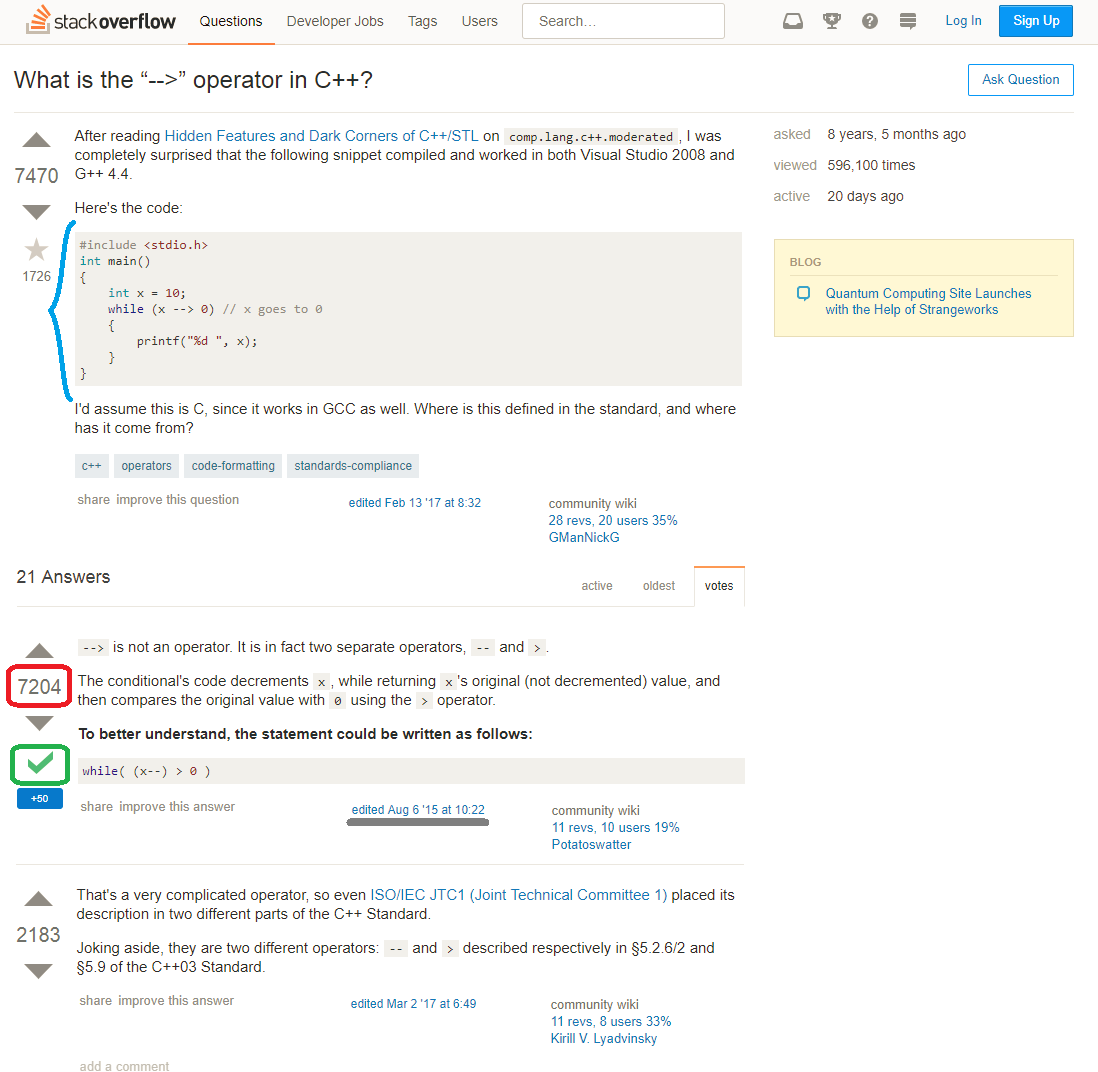
\includegraphics[width=0.95\textwidth]{images/stackoverflow_screen.png}
        \end{center}
    \end{column}
\end{columns}

\end{frame}

%-------------------------------------------------------------------------------

\begin{frame}
\frametitle{Введение}
\framesubtitle{Постановка задачи}

Проблемы:
\begin{itemize}
	\item Большая доля "неразрешенных" вопросов
	\item Нет возможности помочь оценить правильность ответов пользователю, задавшему новый вопрос
\end{itemize}

\vskip0.5cm

Хотим научиться определять правильные ответы, используя базу вопросов StackOverflow

\end{frame}

%-------------------------------------------------------------------------------

\begin{frame}
\frametitle{Введение}
\framesubtitle{Google \& StackOverflow}

\begin{figure}
	\begin{subfigure}[b]{0.49\linewidth}
		\centering
		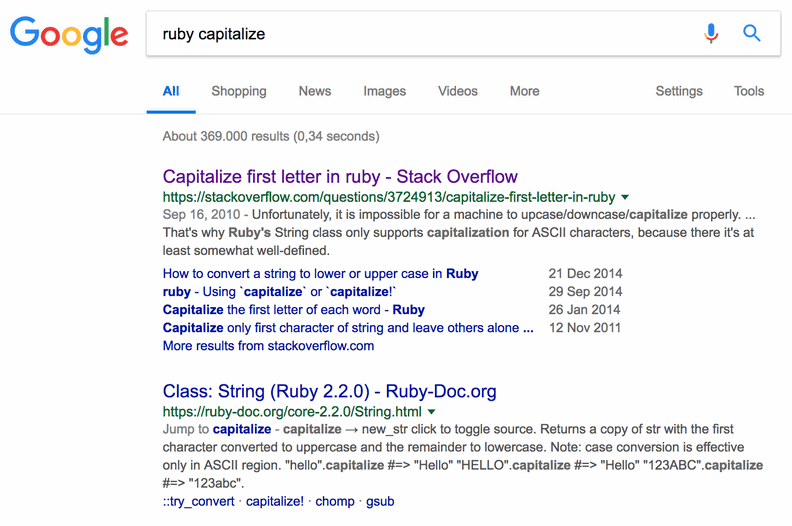
\includegraphics[width=\linewidth]{images/google_search_old.png}
		\caption{Old version}
	\end{subfigure}\hfill
	\begin{subfigure}[b]{0.49\linewidth}
		\centering
		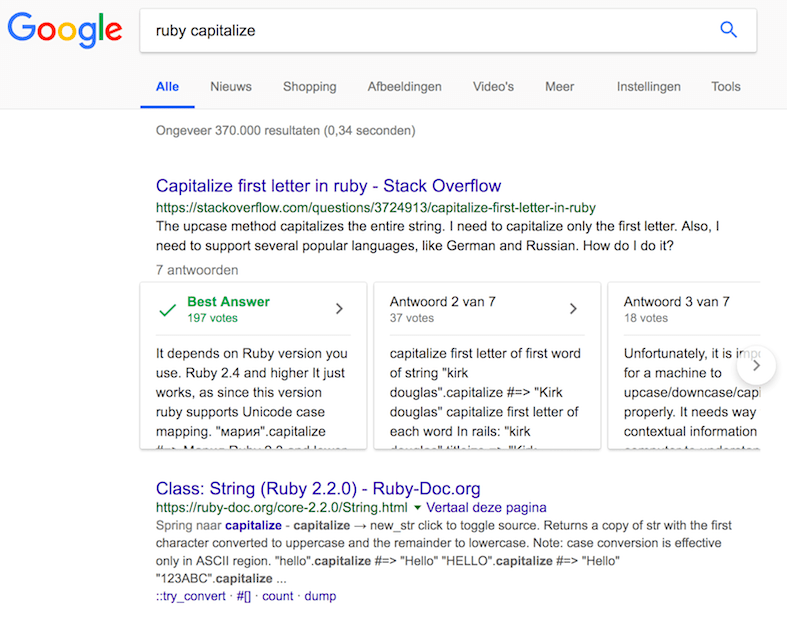
\includegraphics[width=\linewidth]{images/google_search_new.png}
		\caption{New version}
	\end{subfigure}
\end{figure}

\end{frame}

%-------------------------------------------------------------------------------

\begin{frame}
\frametitle{Введение}
\framesubtitle{Обзор имеющихся решений}

"Towards Predicting the Best Answers in CB QAS" (Tian et al. 2013)
\begin{itemize}
	\item Три вида фичей: $A \leftrightarrow A$, $A \leftrightarrow Q$, $A$
	\item Использование Vector Space Model + TF-IDF для определения похожести
	\item Использование лингвистических фичей (длина текста, количество предложений, читаемость и др.)
	\item Учитывается лишь наличие/отсутствие сниппетов кода
	\item Random Forest Classifier
\end{itemize}

\end{frame}

%-------------------------------------------------------------------------------

\begin{frame}
\frametitle{Введение}
\framesubtitle{Обзор имеющихся решений}

"State of the art Best Answer Prediction based on Discretisation of Shallow Linguistic Features" (Gkotsis et al. 2014), 

"Moving to Stack Overflow: Best-Answer Prediction in Legacy Developer Forums" (Calefato et al. 2016)
\begin{itemize}
	\item Четыре вида фичей: $A \leftrightarrow A$, $A$, $user$-$rating$ и $answer$-$rating$, $thread$
	\item Использование лингвистических фичей (длина текста, количество предложений, читаемость и др.)
	\item Использование вероятностной униграмной модели для оценки вероятности ответа
	\item Использование группировки ответов и дискретизации фичей
	\item Не учитывает сниппеты кода
	\item Alternating Decision Tree Classifier
\end{itemize}

\end{frame}

%-------------------------------------------------------------------------------

\begin{frame}
\frametitle{Введение}
\framesubtitle{Минусы имеющихся решений}

\begin{itemize}
	\item Не используется текст вопроса
	\item Не учитывается порядок слов в предложении
	\item Не учитываются синонимы и похожие слова, то есть игнорируется семантика
	\item Не используется содержание сниппетов кода
\end{itemize}

\end{frame}


%-------------------------------------------------------------------------------

\begin{frame}
\frametitle{Цели и задачи}
%\framesubtitle{}

Цель: научиться определять правильность ответа на StackOverflow, используя как его текст, так и код, который может присутствовать внутри ответа

\medskip

Задачи:
\begin{itemize}
	\item Реализовать классификатор на основе нейронных сетей, использующий текст ответов
	\item Добавить использование сниппетов кода в классификаторе 
	\item Сравнить результаты с имеющимися работами
	\item Проанализировать влияние наличия фичей от сниппетов кода на точность классификации
\end{itemize}


\end{frame}

%-------------------------------------------------------------------------------

\begin{frame}
\frametitle{Данные}
\framesubtitle{Общие факты}

Данные:

\begin{itemize}
	\item Дамп базы вопросов StackOverflow
	\item \texttt{XML}-файл размером $\sim50GB$
	\item Новые данные могут быть получены с помощью \texttt{API}
	\item Формат файла: $type\_id$, $id$, $score$, $date$, $body$
\end{itemize}

\end{frame}

%-------------------------------------------------------------------------------

\begin{frame}
\frametitle{Данные}
\framesubtitle{Анализ и обработка}

Анализ:
\begin{itemize}
	\item $40$ миллионов постов, из них $16$ миллионов вопросов и $24$ миллионов ответов
	\item $7$ миллионов вопросов $(47\%)$ без отмеченного правильного ответа
	\item $2$ миллиона вопросов $(13\%)$, у которых нет ни одного ответа
	\item $21.5$ миллионов постов $(54\%)$, в которых присутствуют сниппеты кода. 
\end{itemize}

Обработка:
\begin{itemize}
	\item Удаляем вопросы с рейтингом $\leqslant 0$, а также вопросы, у которых нет ни одного ответа
	\item Из остальных постов извлекаем его $body$
	\item Сохраняем весь код, находящийся в тегах \textless $code$ \textgreater
	\item Очищаем от тегов и сохраняем весь остальной текст вопроса/ответа
\end{itemize}

После обработки получили $6.5$ миллионов вопросов, из них $2$ миллиона вопросов $(31\%)$ без правильного ответа, а также $13.5$ миллионов ответов

\end{frame}

%-------------------------------------------------------------------------------

\begin{frame}
\frametitle{Подходы к анализу текста}
\framesubtitle{Bag of words}

Идея:
\begin{itemize}
    \item Каждому слову сопоставляем вектор длины, равной размеру словаря
	\item Документ: сумма векторов слов
\end{itemize}
Проблемы:
\begin{itemize}
    \item Не учитывается семантика
    \item Не учитывается порядок слов
	\item Большая размерность
\end{itemize}

\end{frame}

%-------------------------------------------------------------------------------

\begin{frame}
\frametitle{Подходы к анализу текста}
\framesubtitle{Bag of words (пример)}

\begin{center}
	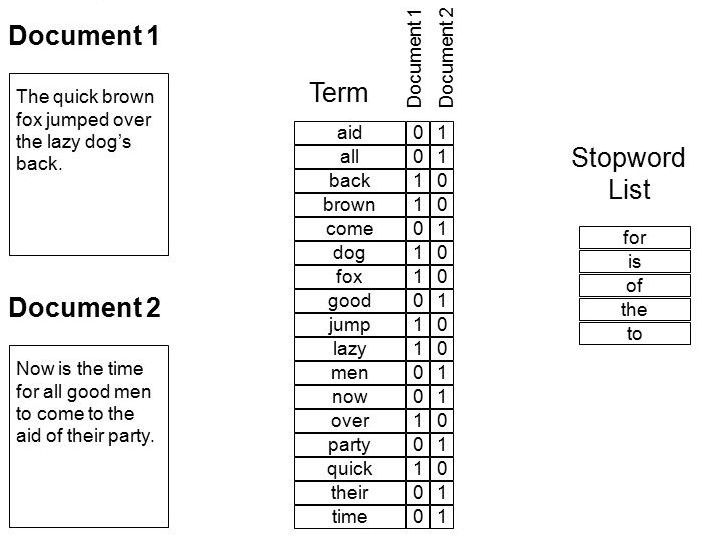
\includegraphics[width=0.7\textwidth]{images/bag_of_words.jpg} 
\end{center}

\end{frame}

%-------------------------------------------------------------------------------

\begin{frame}
\frametitle{Подходы к анализу текста}
\framesubtitle{Word2Vec}

\begin{columns}
    \begin{column}{0.5\textwidth}
    	Идея:
    	\begin{itemize}
        	\item Каждому слову сопоставляем вектор фиксированной длины
        	\item Обучаем на неразмеченном корпусе текстов CBOW/Skip-gram архитектуру        
        	\item Вектор отражает смысл слова, сохраняется семантика
        \end{itemize}

        Чтобы учесть специфику технического языка, обучаться лучше на текстах StackOverflow
    \end{column}
    \begin{column}{0.5\textwidth}
        \begin{center}
            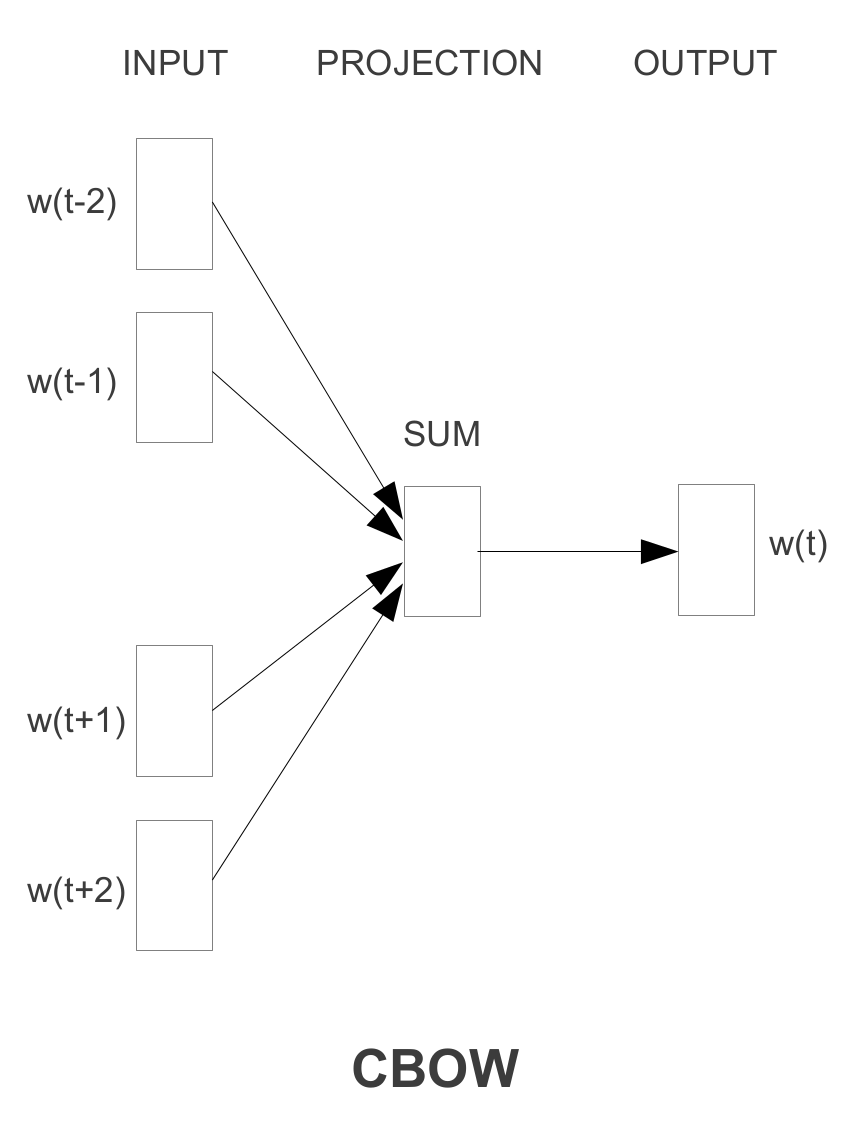
\includegraphics[width=0.9\textwidth]{images/cbow.png} 
        \end{center}
    \end{column}
\end{columns}
\end{frame}

%-------------------------------------------------------------------------------

\begin{frame}
\frametitle{Подходы к анализу текста}
\framesubtitle{Рекуррентные нейронные сети}

Хотим научиться учитывать порядок слов в тексте
    	
Идея:
\begin{itemize}
	\item Используем embedding слов из Word2Vec
	\item Отдаем на вход клетке сети новое слово и выход с предыдущей (учет контекста)
	\item Хотим, чтобы выход сети отражал смысл входного текста
\end{itemize}

Одна из двух основных архитектур: $LSTM$-клетка

Также используются двунаправленные рекуррентные нейронные сети для захвата контекста справа

\begin{center}
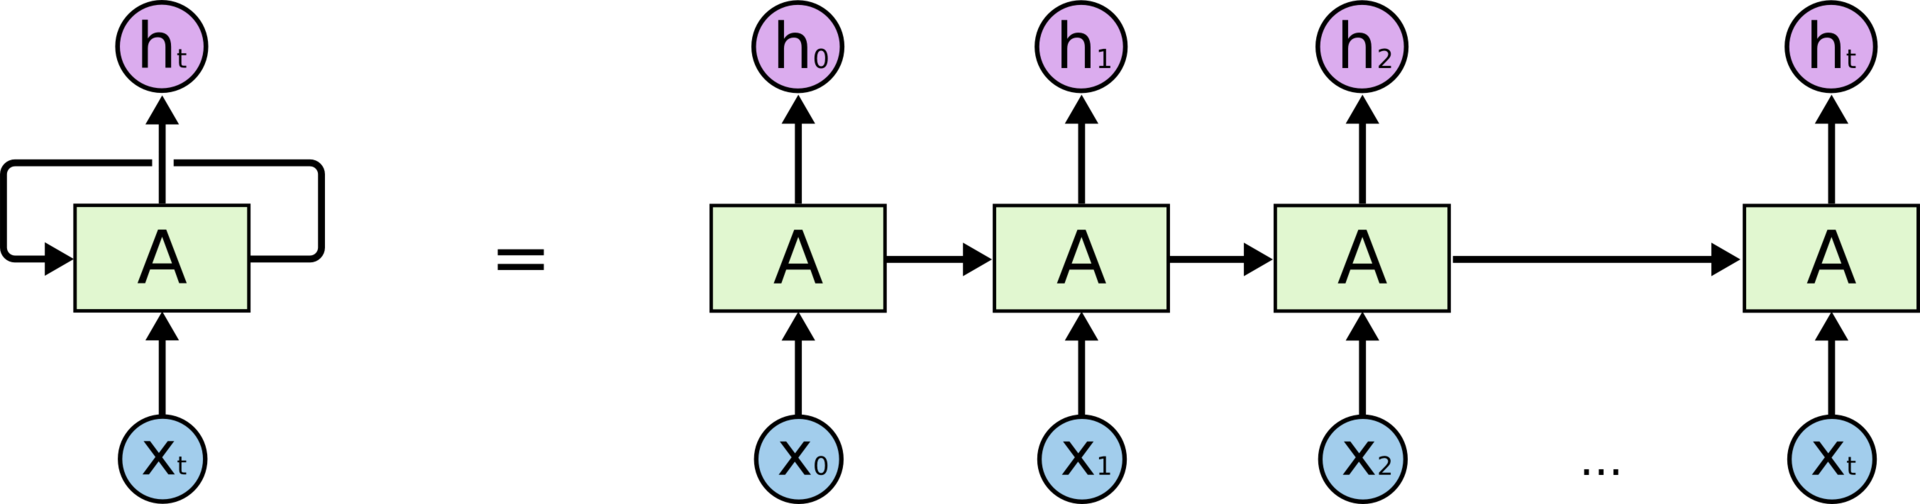
\includegraphics[width=0.7\textwidth]{images/rnn.png}
\end{center}

\end{frame}

%-------------------------------------------------------------------------------

\begin{frame}
\frametitle{Классификация текстов}
\framesubtitle{Базовая архитектура}

\begin{itemize}
	\item Классификация ответов на два класса: правильный/неправильный
	\item В качестве embedding-а используется векторное представление, обученное на текстах вопросов и ответов StackOverflow
\end{itemize}

\begin{center}
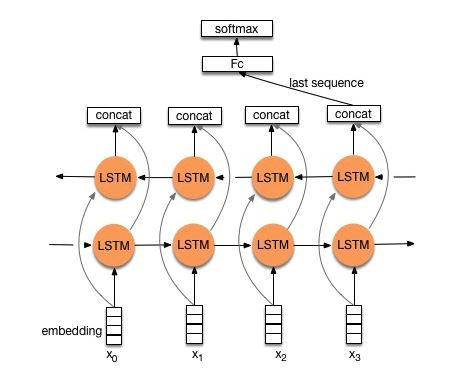
\includegraphics[width=0.6\textwidth]{images/bilstm_text_classification.jpg}
\end{center}

\end{frame}

%-------------------------------------------------------------------------------

\begin{frame}
\frametitle{Классификация ответов}
\framesubtitle{Учет текста вопроса}

\begin{itemize}
	\item Хотим также учитывать текст вопроса, чтобы понимать релевантность ответа
	\item Добавим $BiLSTM$-сеть для текста вопроса и будем использовать эти признаки вместе с признаками ответа 
\end{itemize}

\begin{center}
	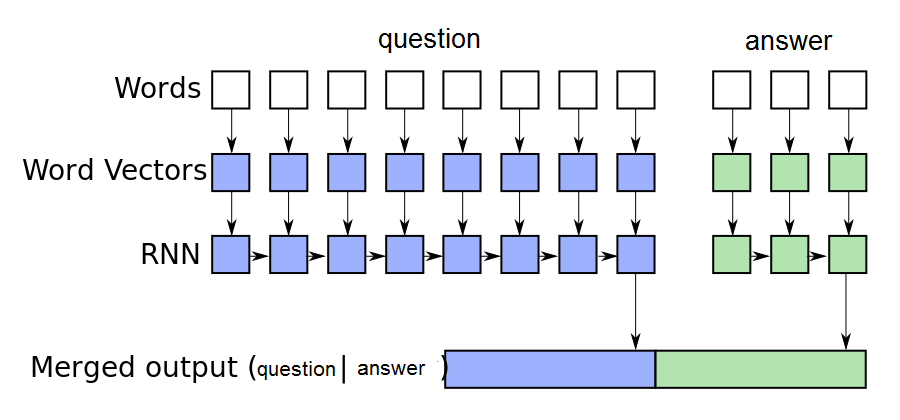
\includegraphics[width=0.6\textwidth]{images/qa.png}
\end{center}

\end{frame}

%-------------------------------------------------------------------------------

\begin{frame}
\frametitle{Подходы к анализу кода}
\framesubtitle{Проблемы}

Код похож на текст, поэтому можно попробовать применить аналогичные методы

Проблема: нелинейная структура кода (циклы, ветвления и др.)

\medskip

\footnotesize{Замечание: тем не менее, может хорошо сработать для однострочных сниппетов}

\end{frame}

%-------------------------------------------------------------------------------

\begin{frame}
\frametitle{Подходы к анализу кода}
\framesubtitle{Использование синтаксического дерева}

(Mou et al., 2014)

\begin{columns}
    \begin{column}{0.6\textwidth}
		Идея:
        \begin{itemize}
			\item Вместо текста кода рассмотрим его синтаксическое дерево
			\item Обучаем Code2Vec, используя в качестве контекста сыновей в синтаксическом дереве
			\item Нормализуем вектора сыновей по размеру их поддерева
		\end{itemize}
    \end{column}
    \begin{column}{0.4\textwidth}
        \begin{center}
            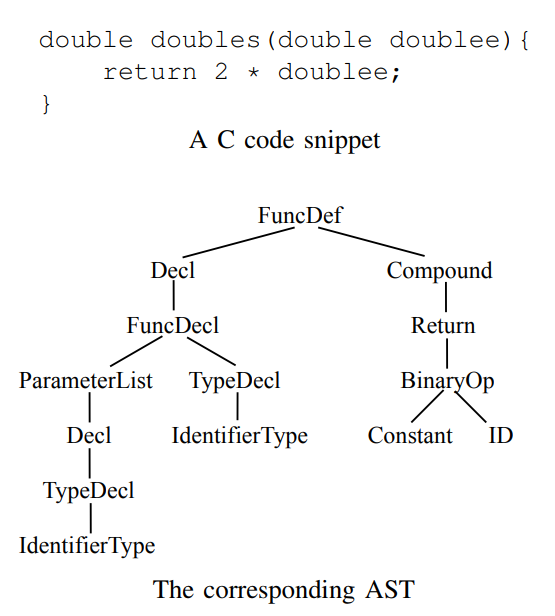
\includegraphics[width=0.9\textwidth]{images/ast.png} 
        \end{center}
    \end{column}
\end{columns}

\end{frame}

%-------------------------------------------------------------------------------

\begin{frame}
\frametitle{Подходы к анализу кода}
\framesubtitle{Использование метода}

\begin{itemize}
	\item Обучаем модель на корпусе кода фиксированного языка программирования (например, \texttt{Python})
	\item В качестве embedding-ов вершин синтаксического дерева используем полученные векторные представления 
	\item Используем RNN, как в случае текста, отдавая на вход полученные embedding-и в порядке обхода $dfs$-ом
\end{itemize}

\end{frame}

%-------------------------------------------------------------------------------

\begin{frame}
\frametitle{Выводы}
\framesubtitle{Результаты}

\begin{itemize}
	\item *сравнение с имеющимися решениями*
	\item Анализ того, какие текстовые представления работают лучше всего
	\item Анализ того, как улучшилась классификация после добавления учета содержания сниппетов кода
\end{itemize}

\end{frame}

%-------------------------------------------------------------------------------
\begin{frame}
\frametitle{Ссылки}
\framesubtitle{Статьи}

\begin{enumerate}
    \item \begin{thebibliography}{99}
            \bibitem[Tian, 2013]{p1} Tian et al. (2013)
            \newblock \href{http://www.public.asu.edu/~bli24/Papers/ICWSM2013.pdf}{Towards Predicting the Best Answers in Community-Based Question-Answering Services}
        \end{thebibliography}
    \item \begin{thebibliography}{99}
            \bibitem[Gkotsis, 2014]{p1} Gkotsis et al. (2014)
            \newblock \href{https://dl.acm.org/citation.cfm?id=2615569.2615681}{It’s all in the Content: State of the art Best Answer Prediction based on Discretisation of Shallow Linguistic Features}
        \end{thebibliography}
    \item \begin{thebibliography}{99}
            \bibitem[Calefato, 2016]{p1} Calefato et al. (2016)
            \newblock \href{https://dl.acm.org/citation.cfm?id=2962585}{Moving to Stack Overflow: Best-Answer Prediction in Legacy Developer Forums}
        \end{thebibliography}
    \item \begin{thebibliography}{99}
            \bibitem[Mou, 2014]{p1} Mou et al. (2014)
            \newblock \href{https://arxiv.org/abs/1409.3358}{Building Program Vector Representations for Deep Learning}
        \end{thebibliography}
\end{enumerate}

\end{frame}


%-------------------------------------------------------------------------------
%	END PRESENTATION SLIDES
%-------------------------------------------------------------------------------

\end{document}